\documentclass[a4paper,11pt]{article}
\usepackage[usenames,dvipsnames]{xcolor}
\usepackage{amsmath,amsthm,amssymb}
\usepackage[margin=2.5cm]{geometry}
\usepackage{ae,aecompl}
\usepackage[utf8]{inputenc}
\usepackage{textcomp}
\usepackage{natbib}
\usepackage{sgame}
\usepackage[onehalfspacing]{setspace}
\usepackage{graphicx}
\usepackage{tikz}

\newtheorem{definition}{Definition}
\newtheorem{lemma}{Lemma}
\newtheorem{proposition}{Proposition}
\newtheorem{theorem}{Theorem}
\newtheorem{claim}{Claim}
\newtheorem{example}{Example}
\newtheorem{corollary}{Corollary}

\title{Advanced Microeconomics II\\ Solution sketches for exercises not covered in class}
\author{Christoph Schottmüller}
\begin{document}
\maketitle

\section{Nash theorem}
\label{sec:nash-theorem}

\paragraph{Continuity of the best response in exercise 1:} We saw that continuity of $u_i$ and the compactness of the strategy set imply existence of a best response and that strict quasiconcavity implies uniqueness of the best response. Let me show a bit more formally that the best response function is continuous. This is a proof by contradiction. Therefore, suppose that the best response function $s_i^*$ is discontinuous at some $s_{-i}$. This implies that there is a sequence of $\{s_{-i}^k\}_{k=1}^\infty$ converging to $s_{-i}$ such that $|s_{i}^*(s_{-i}^k)-s_i^*(s_{-i})|>\varepsilon $ for some $\varepsilon >0$ and all $k=1,2,\dots$. As the sequence $\{s_i^*(s_{-i}^k)\}_{k=1}^{\infty}$ has all its elements in the compact set $[0,1]$, it has a converging subsequence. Denote this subsequence by $\{ b^k\}_{k=1}^\infty$ and the corresponding sequence of $s_{-i}^k$ to which the $b^k$ are best responses by $\{a^k\}_{k=1}^\infty$ (this is a subsequence of  $\{s_{-i}^k\}_{k=1}^\infty$) . Let $b=\lim_{k\rightarrow\infty}b^k$ and let us, for simplicity, first assume that $b$ is interior, i.e. $b\in(0,1)$. Then $b^k$ are interior for sufficiently high $k$ and for these the first order condition
$$\frac{\partial u_i}{\partial s_i }(b^k,a^k)=0$$
has to be satisfied. Hence,
$$\lim_{k\rightarrow\infty}\frac{\partial u_i}{\partial s_i }(b^k,a^k)=0$$
(as the limit of a sequence of zeros is simply zero).
By the continuity of $\partial u_i/\partial s_i$ in both of its arguments
$$\lim_{k\rightarrow\infty}\frac{\partial u_i}{\partial s_i }(b^k,a^k)=\frac{\partial u_i}{\partial s_i }(\lim_{k\rightarrow\infty}b^k,\lim_{k\rightarrow\infty}a^k)$$
and therefore
$$\frac{\partial u_i}{\partial s_i }(\lim_{k\rightarrow\infty}b^k,\lim_{k\rightarrow\infty}a^k)=0.$$
This implies that $b=\lim_{k\rightarrow\infty}b^k$ is the best response to $\lim_{k\rightarrow\infty}a^k=s_{-i}$. But this contradicts that all $b^k$ (and therefore also their limit) are at least $\varepsilon>0 $ away from $s_i^*(s_{-i})$ (recall that our assumptions implied that the best response is unique!).\footnote{The case where $b$ is not interior works similarly: Still the first order condition (now possibly in inequality form) has to hold for every $k$ and therefore also in the limit. Continuity of $\partial u_i/\partial s_i$ allows to take the limits inside the first order condition and gives the result that the limit $b^k$ is the best response to the limit $a^k$.}


\section{Auctions}
\label{sec:auctions}

\paragraph{Addendum to the double auction  (exercise 2).} We derived the equilibrium in linear bidding strategies as
\begin{eqnarray*}
  b_b(v)&=&\frac{2}{3}v+\frac{1}{12}\\
  b_s(c)&=&\frac{2}{3}c+\frac{1}{4}.
\end{eqnarray*}
Note that trade takes place if and only if the buyer's bid is above the seller's bid, that is if and only if $b_b(v)-b_s(c)\geq 0$ which is equivalent to $2/3 (v-c)-2/12\geq 0$ or equivalently $v-c\geq 1/4$. That is, the equilibrium of the double auction is such that trade only occurs if the gains from trade exceed $1/4$ (while efficiency would require trade whenever the gains from trade exceed 0).

Some technical notes: Note that buyers with type $v\in[0,1/4]$ bid below $1/4$ and therefore below the bid of the lowest seller type. Put differently, buyers with type $v\in[0,1/4]$ have probability zero of trading. Their expected payoff in equilibrium is therefore zero although their bid is above their valuation (which admittedly looks a bit strange at first sight). You may now realize that, strictly, speaking we misspecified the expected payoff that we used to derive the best response function. We wrote this as
\begin{equation*}
  \frac{b_b-\gamma}{\delta}\left[v-\frac{1}{2}b_b-\frac{1}{2}\frac{\gamma+b_b}{2}\right].
\end{equation*}
For bids below $\gamma=1/4$, however, the probability of trade is not $(b_b-\gamma)/\delta$ but zero (also the trading price conditional on trading is not really defined for such low bids as trade never occurs when bidding so low). That is, expected payoff equals the expression above if $b_b\in[\gamma,\gamma+\delta]$ and 0 if $b_b<\gamma$ (and 1 if $b_b>\gamma+\delta$ but this will not be relevant). Note that the derived solution is nevertheless correct: For $v>\gamma$, the first order condition is still correct and these types make a positive expected payoff in equilibrium (as they trade with positive probability and their bid is below their valuation) and will therefore not want to deviate to bids that give zero probability of trade implying zero payoff. Now turn to $v\leq \gamma$. For $b_b\in[\gamma,\gamma+\delta]$, it is straighforward to check that the buyer's expected payoff is concave in $b_b$ (just verify that the second derivative is negative). Furthermore, the derivative of the expected payoff with respect to $b_b$ at the point $b_b=\gamma$ equals $v-\gamma$. That is, if $v<\gamma$, then the first derivative is negative at the point $b_b=\gamma$ and by concavity it is then also negative for $b_b>\gamma$. Put differently, the expected payoff of a type $v<\gamma$ is decreasing over the range of bids that yield trade with positive probability. Hence, it is optimal for a buyer with $v<\gamma$ to bid such that his expected probability of trade is zero and bidding according to the linear bidding function that we derived is one way of doing exactly that.

\paragraph{Contest (exercise 3).} We derive a symmetric equilibrium in strictly decreasing and differentiable strategies. Assume that such an equilibrium exists and is given by the strategy $s:[0.1,1.1]\rightarrow \Re_+$ with inverse $t$. The maximization problem of a contestant given that the other contestant uses the strategy $s$ is
\begin{equation*}
  \max_e prob[e>s(\theta _j)]-e\theta _i
\end{equation*}
which is equivalent to 
\begin{equation*}
  \max_e prob[t(e)<\theta _j]-e\theta _i
\end{equation*}
as $s$ and therefore also its inverse $t$ are strictly decreasing by assumption. By the assumption that $\theta _j$ is uniformly distributed on $[0.1,1.1]$ the maximization problem can be written as
\begin{equation*}
  \max_e 1.1-t(e)-e\theta _i.
\end{equation*}
The first order condition to this maximization problem is
\begin{equation*}
  -t'(e)-\theta _i=0.
\end{equation*}
In a symmetric equilibrium, the optimal effort decision by type $\theta _i$ at which this first order condition holds is $s(\theta _i)$ and therefore the first order condition becomes then
\begin{equation*}
  -\frac{1}{s'(\theta _i)}-\theta _i=0
\end{equation*}
or equivalently
\begin{equation*}
  -s'(\theta _i)=1/\theta _i.
\end{equation*}
In a symmetric equilibrium with $s$ strictly decreasing in type, the highest possible type, i.e. 1.1, has a zero probability of winning the price and should therefore optimally bid 0. That is, $s(1.1)=0$ in such an equilibrium. This initial condition yields together with $-s'(\theta _i)=1/\theta _i$ the solution
\begin{equation*}
  s(\theta _i)=\int_{\theta _i}^{1.1}1/x \;dx=log(1.1)-log(\theta _i).
\end{equation*}
The inverse $t$ is then
\begin{equation*}
t(s)=e^{log(1.1)-s}.
\end{equation*}
(To verify that this is indeed an equilibrium we should check that also the second order condition is satisfied in the maximization problem above with this function $t$. Indeed the second derivative equals $-e^{log(1.1)-s}<0$.)

\section{SPNE}
\label{sec:spne}

Take one of the subgames of $\Gamma_E$ starting after $T-1$ repetitions, i.e. a subgame consisting of the last repetition after some history . Note that this is indeed a subgame as each player is informed about all moves of all other players in previous rounds. Therefore, we do not cut through information sets. This subgame is equivalent to $\Gamma$ with the exception that each player's payoff is increased by some constant equal to the payoff from previous rounds. As this increase is constant, i.e. it does not depend on the choice of strategies in the subgame, it does not affect best responses or equilibrium. Therefore, the unique equilibrium in the subgame is $\sigma$ (as $\sigma$ is the unique equilibrium in $\Gamma$ by assumption). This establishes that in the last repetition $\sigma$ is played in every SPNE of $\Gamma_E$ (regardless of play in repetitions $1,\dots,T-1$).

The proof works through backwards induction. The statement we have to show is the following: \emph{If $\sigma$ is played in all SPNE of $\Gamma_E$ in repetitions $t=t'+1,\dots,T$, then $\sigma$ is also played in all SPNE in repetition $t'$.} To show this, suppose  $\sigma$ is played in all SPNE of $\Gamma_E$ in repetitions $t=t'+1,\dots,T$ and take some subgame in repetition $t'$. Payoffs of player $i$ in SPNE as a function of his decision and the decision of the other players in $t'$ equals
\begin{equation*}
  u_i^{t'}=u_i(\sigma_i^{t'},\sigma_{-i}^{t'})+(T-t')u_i(\sigma)+const
\end{equation*}
as in all of the following $T-t'$ following periods $\sigma$ is played by the induction hypothesis and $const$ denotes the payoffs from earlier periods ($1,\dots,t'-1$). That is, the subgame is in fact equivalent to $\Gamma$ with the only difference that payoffs are shifted by a constant for each player -- namely $(T-t')u_i(\sigma)+const$. As such a shift does not affect best responses, the equilibria in the subgame are the same as the equilibria in $\Gamma$ which implies that $\sigma$ is played in the subgame in every SPNE. This establishes the claim in italics. In combination with the  result that $\sigma$ is played in repetition $T$, this proves the result.

\paragraph{Extra exercise.} Let $\Gamma$ be the game below with the unique Nash equilibrium ($M$,$C$) and let $T=2$. 
\begin{center}
\begin{game}{3}{3}
& $L$ & $C$  & $R$ \\
$T$ & 2,2 & 0,3 &-10,-10\\
$M$&  3,0    & 1,1  & -10,-10  \\
$B$ & -10,-10 & -10,-10 & -11,-11
\end{game}
\end{center}


Let player 1 (2) choose the following strategy in $\Gamma_E$: Play $T$ ($L$) in period 1. If the other player chose $L$ ($T$) in period 1, then play $M$ ($C$) in period 2. Otherwise, play $B$ ($R$) in period 2. It is easily checked that this is a NE of $\Gamma_E$ but not a SPNE.

\section{Screening}
\label{sec:screening}

Exercise 3: Denote the costs of producing quantity $q$ by type $\theta $ as $c(q,\theta )$. Hence, $U(\theta )=t(\theta )-c(q(\theta ),\theta )$ and the envelope theorem states that in every incentive compatible mechanism $U'(\theta )=-c_\theta (q(\theta ),\theta )$ for almost all types.\footnote{ More precisely, incentive compatibility requires
  \begin{eqnarray*}
    U(\theta )&\geq& U(\theta ')+c(q(\theta '),\theta ')-c(q(\theta '),\theta )\\
    U(\theta' )&\geq& U(\theta )+c(q(\theta ),\theta )-c(q(\theta ),\theta' )
  \end{eqnarray*}
  which can (let $\theta >\theta '$) be rearranged to
  \begin{equation*}
    \frac{-(c(q(\theta ),\theta )-c(q(\theta ),\theta'))}{\theta -\theta'} \geq \frac{U(\theta )-U(\theta')}{\theta -\theta '}\geq \frac{-(c(q(\theta '),\theta )-c(q(\theta '),\theta '))}{\theta -\theta'}.
  \end{equation*}
   Take the limit as $\theta '\rightarrow\theta $ to get $U'(\theta )=-c_\theta (q(\theta ),\theta )$ at types where $q$ is continuous. Note that the two outer inequalities chained together can be written as $\int_{\theta '}^\theta  c_\theta (q(\theta '),x)-c(q(\theta ),x)\,dx\geq 0$ or equivalently $\int_{\theta '}^\theta \int_{q(\theta ')}^{q(\theta )}-c_{q\theta }(y,x)\,dy\,dx\geq 0$. If $c_{q\theta }(q(\theta ),\theta )<0$ (and $q$ is continuous at $\theta $), this implies that $q$ has to be increasing in a neighborhood around $\theta $ as otherwise the inequality could not hold for $\theta '$ close to $\theta $.
}
  Put differently,
\begin{equation*}
  U(\theta )=U(1/4)+\int_{1/4}^\theta -c_\theta (q(x),x)\,dx.
\end{equation*}
Incentive compatibility between $\theta =1/2$ and $\theta =1/4$ requires that 
\begin{equation*}
  U(1/2)\geq U(1/4)+c(q(1/4),1/4)-c(q(1/4),1/2)
\end{equation*}
which -- using the envelope theorem above with $\theta =1/2$ -- can be rewritten as 
\begin{equation*}
  \int_{1/4}^{1/2} -c_\theta (q(x),x)\,dx\geq c(q(1/4),1/4)-c(q(1/4),1/2)
\end{equation*}
which is equivalent to 
\begin{equation*}
  \int_{1/4}^{1/2} -c_\theta (q(x),x)\,dx\geq -\int_{1/4}^{1/2} c_\theta (q(1/4),x)\; dx
\end{equation*}
or 
\begin{equation*}
  \int_{1/4}^{1/2} c_\theta (q(1/4),x)-c_\theta (q(x),x)\,dx\geq 0
\end{equation*}
which is equivalent to
\begin{equation}
  \label{eq:6}
  \int_{1/4}^{1/2}\int_{q(1/4)}^{q(x)} -c_{q\theta} (y,x)\,dy\,dx\geq 0.
\end{equation}
For the cost function $c(q,\theta )=\theta  q-q^2/(2\theta )-\theta /5+constant$, the cross derivative is $c_{q\theta }(q,\theta )=1-q/\theta ^2$. If we use $q(\theta )=\theta ^2+\varepsilon $ (for some small $\varepsilon >0$) it is clear that the integrand in (\ref{eq:6}) is mostly negative and therefore the inequality (\ref{eq:6}) cannot be satisfied. (Note, however, that the monotonicity condition derived in the previous footnote, i.e. $q$ has to be increasing if $c_{q\theta }(q(\theta ),\theta )<0$ is satisfied.)

\begin{figure}[h]
  \centering
  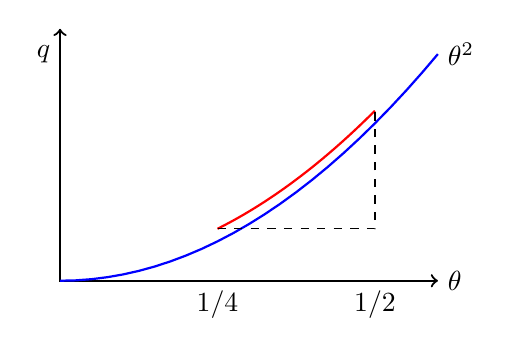
\begin{tikzpicture}[scale=8]
    \draw[thick,<->] (0,0.4)--(0,0)--(0.6,0);
    \draw[blue, thick, domain=0:0.6] plot (\x, {\x*\x});
    \draw[red, thick, domain=0.25:0.5] plot (\x, {\x*\x+0.02});
    \node[right] at (0.6,0.36){$\theta^2$};
    \node[right] at (0.6,0){$\theta$};
    \node[left] at (0,0.36){$q$};
    \node[below] at (0.25,0){$1/4$};
    \node[below] at (0.5,0){$1/2$};
    \draw[dashed] (0.25,1/16+0.02)--(0.5,1/16+0.02)--(0.5,0.27);
  \end{tikzpicture}
  \caption{Illustration screening exercise 3: above (below) $\theta ^2$ we have $c_{q\theta }<(>)0$. The double integral in (\ref{eq:6}) integrates over the triangular area given by the dashed lines and the red curve which depicts $q(\theta )=\theta ^2+\varepsilon $.}
  \label{fig:nosc}
\end{figure}
\par
This illustrates that the combination of envelope theorem and a monotonicity condition is only equivalent to incentive compatibility if the so called ``single crossing condition'' is satisfied, i.e. only if $c_{q\theta }$ has the same sign for all $(q,\theta )$ pairs. 

\end{document}